\documentclass[a4paper, 12pt]{article}%тип документа

%отступы
\usepackage[left=2cm,right=2cm,top=2cm,bottom=3cm,bindingoffset=0cm]{geometry}

%Русский язык
\usepackage[T2A]{fontenc} %кодировка
\usepackage[utf8]{inputenc} %кодировка исходного кода
\usepackage[english,russian]{babel} %локализация и переносы

%Вставка картинок
\usepackage{wrapfig}
\usepackage{graphicx}
\graphicspath{{pictures/}}
\DeclareGraphicsExtensions{.pdf,.png,.jpg}

%оглавление
\usepackage{titlesec}
\titlespacing{\chapter}{0pt}{-30pt}{12pt}
\titlespacing{\section}{\parindent}{5mm}{5mm}
\titlespacing{\subsection}{\parindent}{5mm}{5mm}
\usepackage{setspace}

%Графики
\usepackage{multirow}
\usepackage{pgfplots}
\pgfplotsset{compat=1.9}

%Математика
\usepackage{amsmath, amsfonts, amssymb, amsthm, mathtools}

%Стиль страницы
\usepackage{fancyhdr}
\pagestyle{fancy}

\begin{document}

\begin{titlepage}

\begin{center}
%\vspace*{1cm}
\large\textbf{Московский Физико-Технический Институт}\\
\large\textbf{(государственный университет)}
\vfill
\line(1,0){430}\\[1mm]
\huge\textbf{Работа 3.4.2}\\
\line(1,0){430}\\[1mm]
\vfill
\large Сибгатуллин Булат, ФРКТ\\
\end{center}

\end{titlepage}

\fancyhead[L] {Работа 3.4.2}
\noindent \textbf{Цель работы:} \\
\indent Изучение температурной зависимости магнитной восприимчивости ферромагнетика выше точки Кюри\\
\noindent \textbf{В работе используются:} \\
\indent катушка с образцом из гадолиния, термостат, частотомер, цифровой вольтметр, LC-автогенератор, термопара медь-константан.

\section*{Описание работы}

\subsection*{Теоретическая справка}

Ферромагнитики обладают свойством намагничиваться даже в слабых магнитных полях. В настоящей работе для изучения температурной зависимости магнитной восприимчивости ферроматгнетика выше точки Кюри (то есть в парамагнитной области) используется закон Кюри-Вейса:

\begin{equation}
\chi = \frac{C}{T - \Theta_p} \sim \frac{1}{T - \Theta_p},
\end{equation}

где $\chi$ - магнитная восприимчивость, $C$ - постоянная Кюри, зависящая от вещества, $T$ - абсолютная температура, $\Theta_p$ - парамагнитная температура Кюри.

\vspace{0.5cm}

При повышении температуры $T$ возрастает дезориентирующее действие телового движения частиц, и магнитная восприимчивость парамагнетиков убывает, в простейшем случае (в постоянном магнитном поле) - по закону Кюри

%Тут вставить (Теоретический график зависимости обратной магнитной восприимчивости от температуры)
\begin{wrapfigure}{l}{0.4\linewidth} 
	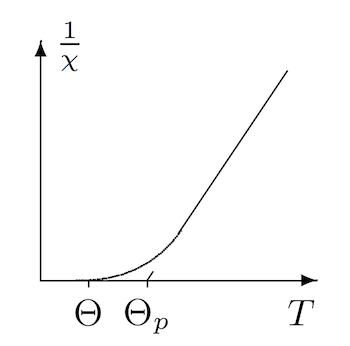
\includegraphics{images/Kury_veis.png}
	\caption{Теоретический график зависимости обратной магнитной восприимчивости от температуры}
\end{wrapfigure}

При $T \rightarrow$ 0 тепловое движиние всё меньше препятствует магнитным моментам атомов ориентироваться в одном направлении при сколь угодно слабом внешнем поле. В ферромагнетиках (под влиянием обменных сил) это происходит при понижении температуры не до абсолютного нуля, а до температуры Кюри $\Theta$, в котором добавка к температуре $\Theta_p$ - некая температура, называемая парамеагнитной точкой Кюри. Она близка к $\Theta$, но немного больше её (рис. 1). Оказывается, что у ферромагнетиков закон Кюри должен быть заменён законом Кюри-Вейсса (1). Эта формула хорошо описывает поведение ферромагнитных вещетсв после их перехода в парамагнитную фазу при заметном удалении температуры от 0, но недостаточно точна при $T \approx \Theta$/

\vspace{0.5cm}

В нашей работе изучается температурная зависимость $\chi (T)$ гадолиния при температурах выше точки Кюри. Выбор материала определяется тем, что его точка Кюри лежит в интервале комнатных температур.

\subsection*{Экспериментальная установка}

%Здесь нужно вставить (Схема экспериментальной установки)
\begin{figure}[h!]
\centering
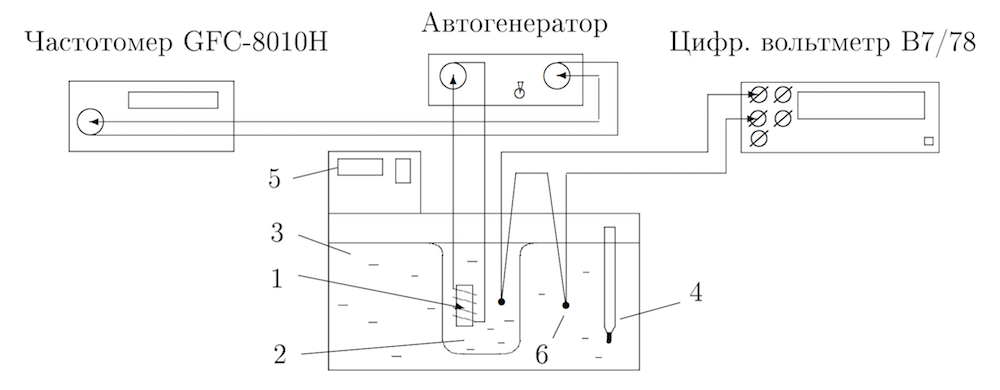
\includegraphics[width=\linewidth]{images/scheme.png}
\caption{Схема экспериментальной установки}
\label{fig:Image2}
\end{figure}

Схема установки для проверки закона Кюри-Вуйерса показана на рис. 2. Исследуемый ферромагнитный образец (гадолиний) расположен внутри пустотулой катушки самоиндукции, которая служит индуктивностью колебательного контура, входящего в состав $LC$-автогенератора.

\vspace{0.5cm}

Гадолиний является хорошим проводником электрического тока, а рабочая частота генератора достаточно велика (50 кГц), поэтому для уменьшения вихревых токов образец изготовлен их мелких кусочков размеров 0,5 мм. Катушка 1 с образцом помещена в стеклянный сосуд 2, залитый трансформаторным маслом. Масло предохраняет образец от окисления и способствует ухудшению электрического контакта между отдельными частичками образца. Кроме того, оно улучшает тепловой контакт между образцом и термостатируемой (рабочей) жидкостью 3 в термостате. Ртутный термометр 4 используется для приближенной оценки температуры. При изменении температуры меняется магнитная восприимчивость образца $\chi$, а следовательно, самоиндукция катушки и период колебаний $\tau$ автогенератора. Для измерения периода используется частотомер.

\vspace{0.5cm}

Закон Кюри-Вейса справедлив, если выполнено соотношение

\[
\frac{1}{\chi} \sim T - \Theta_p \sim \frac{1}{\tau^2 - \tau_0^2},
\]

где $\tau_0$ - период колебаний без образца.

\vspace{0.5cm}

Для нагрева используется термостат. Температура исследуемого образца всегда несколько отличается от температуры дистилированной воды в сосуде. После того, как вода достигла заданной температуры, идёт медленный процесс выравнивания температур образца и воды. Разность их температур контролируется с помощью медноконтантавой трмопары 6 и цифрового вольтметра. Один из спаев термопары находится в тепловом контакте с образцом, а другой погружен в воду. Концы термопары подключены к цифровому вольтметру. Рекомендуется измерять период колебаний автогенератора в тот момент, когда указанная разность температур становится $\leq 0,5^{\circ} C$. Чувствительность термопары $k = 24$ град/мВ.

\section*{Выполнение работы}

\begin{enumerate}

\item Исследуем зависимость периода колебаний $LC$ - генератора от температуры образца. Запишем данные в таблицу:

%Таблица с зависимостью \tau (T)
\begin{figure}[h!]
\centering
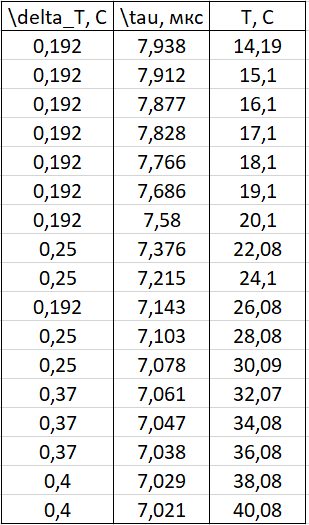
\includegraphics[scale = 1.4]{images/table_t(T).png}
\caption{Зависимость $\tau (T)$}
\label{fig:Image3}
\end{figure}

\item Период колебаний без образца уаказан на установке и равен $\tau_0 = 6,9092 \: \text{мкс}$.

\item По полученным данным построим графики зависимости $f(T) = \tau^2 - \tau^2_0$ и $f(T) = 1/(\tau^2 - \tau^2_0)$.

\begin{figure}[h!]
\centering
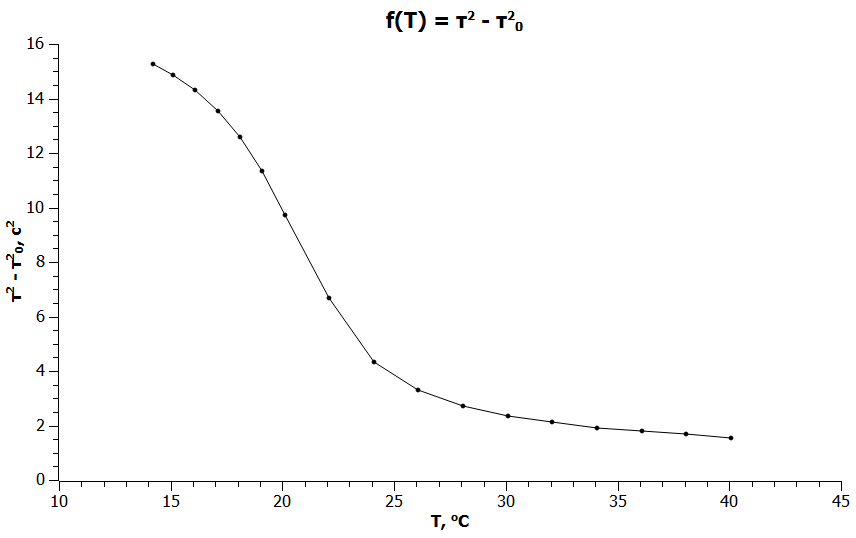
\includegraphics[scale = 0.8]{images/graph1.png}
\caption{$f(T) = \tau^2 - \tau^2_0$}
\label{fig:Image3}
\end{figure}

\begin{figure}[h!]
\centering
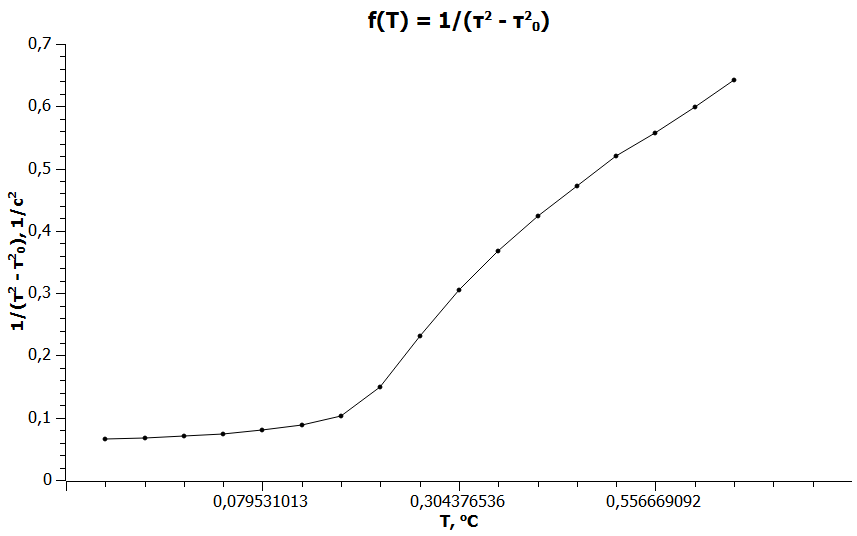
\includegraphics[scale = 0.8]{images/graph2.png}
\caption{$f(T) = 1/(\tau^2 - \tau^2_0)$}
\label{fig:Image3}
\end{figure}

\item Определим парамагнитную точку Кюри для гадолиния:

\[T_1 - \Theta_p = k\frac{1}{\tau^2_1 - \tau^2_0}\]

\[T_2 - \Theta_p = k\frac{1}{\tau^2_2 - \tau^2_0}\]

Преобразуя данные уравнения получаем:

\[\Theta_p = \frac{T_1(\tau^2_1 - \tau^2_0) - T_2(\tau^2_2 - \tau^2_0)}{(\tau^2_1 - \tau^2_0) - (\tau^2_1 - \tau^2_0)}\]

При помощи МНК найдем значение $\Theta_p \simeq = 14,5 \: ^{\circ}C = 287,65 \:K$. Погрешность измерений составила - $\sigma_{\Theta_p} = 5,3 \: K$.

В итоге получаем:

\[\Theta_p = 287,65 \pm 5,3 \: K\]

Сравним с табличным значением: $\Theta_{p \: \text{табл}} = 292 \: K$. Полученные экспериментальным путем результаты сходятся с табличными в пределах погрешности.

\end{enumerate}

\end{document}